\documentclass[tikz,border=8pt]{standalone}
\usetikzlibrary{arrows.meta,calc}

\begin{document}
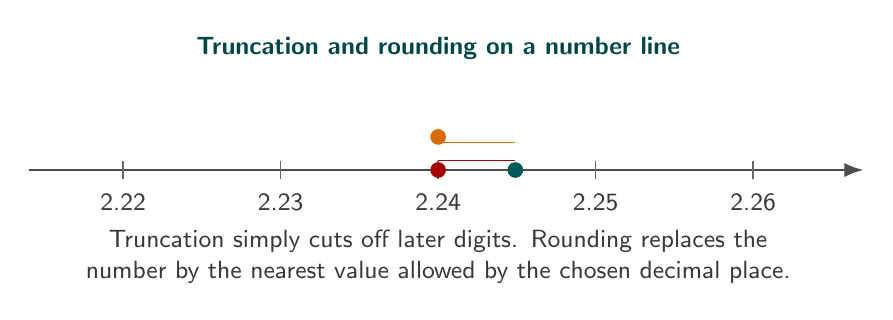
\begin{tikzpicture}[
  axis/.style={-{Latex[length=2.4mm]},draw=black!70,line width=0.75pt},
  tick/.style={draw=black!60,line width=0.55pt},
  label/.style={font=\sffamily\small,text=black!78},
  title/.style={font=\sffamily\bfseries\small,text=teal!55!black},
  point/.style={circle,fill=teal!70!black,inner sep=2pt},
  trunc/.style={circle,fill=red!65!black,inner sep=2pt},
  round/.style={circle,fill=orange!85!black,inner sep=2pt},
]

\node[title] at (0,1.55) {Truncation and rounding on a number line};
\draw[axis] (-5.2,0) -- (5.4,0);
\foreach \x/\lab in {-4/2.22,-2/2.23,0/2.24,2/2.25,4/2.26} {
  \draw[tick] (\x,-0.12) -- (\x,0.12);
  \node[label,below] at (\x,-0.18) {\lab};
}

\node[point,label={[label]above:true value $2.2449$}] at (0.98,0) {};
\node[trunc,label={[label]above left:truncate to $2.24$}] at (0,0) {};
\node[round,label={[label]above right:round to $2.24$}] at (0,0.42) {};
\draw[red!65!black,line width=0.6pt] (0.98,0.12) -- (0,0.12);
\draw[orange!85!black,line width=0.6pt] (0.98,0.35) -- (0,0.35);

\node[label,align=center,text width=9.4cm] at (0,-1.1)
  {Truncation simply cuts off later digits. Rounding replaces the number by the nearest value allowed by the chosen decimal place.};

\end{tikzpicture}
\end{document}
